\section{The basics}

\np Toward playing music, there must be series of musical notes written for the player to read.
For dats, a musical note is declared with the keyword \verb+n+. \verb+n+ must contain two arguments,
a length and a note, each are separated by a comma:


\begin{Verbatim}[frame=single]
       n <length>, <note>;
\end{Verbatim}

%\begin{center}
%\includegraphics{s1.pdf}
%\end{center}

\np an example of such declaration is:
\begin{Verbatim}[frame=single]
       n 4, c4;
\end{Verbatim}

This is a declaration of musical note of length 1/4, playing the note c4. The length
is just the denominator of how much measure the musical note took.

\np Such musical notes, (and musical rests), are always declared inside a \textit{staff block}:

\begin{Verbatim}[frame=single]
      staff foo {
        n 4, c4;
      }
\end{Verbatim}

produces:

\begin{center}
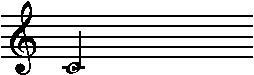
\includegraphics{notes/c4}
\end{center}

\np Now we have a staff, what else do we need? A `main`. A main is basically
where you do your operations on staffs and synthesize, producing sounds.

\np First, we process the staff using a synthesizer. The output of this synthesizer
is then stored into a variable, usually a type of `track`:

\begin{Verbatim}[frame=single]
      staff foo {
        n 4, c4;
      }

      main {
        track bar = synth.kpa(foo);
        write("w.wav", bar);
      }
\end{Verbatim}

\np This is then written into a file named, "w.wav". (Currently, Dats only supports writing wav files.)

\np To append one or more track to another track, you may simply just add a comma, followed by the track
you were appending with:

\begin{Verbatim}[frame=single]
      track tr1 = synth.kpa(/* some staff */);
      track tr2 = synth.kpa(/* some staff */);
      track tr3 = tr1, tr2, tr2;
\end{Verbatim}
